\documentclass{article}
\usepackage[utf8]{inputenc}

\title{Ph20 Set 2 Comments}
\author{Nezir Alic}
\date{February 2019}
\usepackage{graphicx}
\begin{document}

\maketitle

1.) We can derive Simpson's Formula using a Taylor Expansion. First, we find the exact expression by integrating over the interval $(x_0, x_2)$, where $x_2 - x_0 = 2h$ and there exists a midpoint $x_1$ within the interval.
\\
\\
$
\int_{x_0}^{x_1} \! f(x) \, \mathrm{d}x = \int_{x_0}^{x_1} \! [f(x_1) + f'(x)(x - x_1) + {\frac{f''(x_1)}{2!}}(x - x_1)^2 + {\frac{f'''(x_1)}{3!}}(x - x_1)^3 + {\frac{f^{(4)}(\eta)}{4!}}(x - x_1)^4] \, \mathrm{d}x
$
\\ 
\\
$= [f(x_1)x + {\frac{f'(x_1)}{2}}(x - x_1)^2 + {\frac{f''(x_1)}{6}}(x - x_1)^3 + {\frac{f'''(x_1)}{24}}(x - x_1)^4  + {\frac{f^{(4)}(\eta)}{120}}(x - x_1)^5]_{x_0}^{x_1}$
\\
\\
$
= f(x_1)(x_2 - x_1) + {\frac{f'(x_1)}{2}}((x_2 - x_1)^2 - (x_0 - x_1)^2) + {\frac{f''(x_1)}{6}}((x_2 - x_1)^3 - (x_0 - x_1)^3) + {\frac{f'''(x_1)}{24}}((x_2 - x_1)^4 - (x_0 - x_1)^4) + {\frac{f^{(4)}(\eta)}{120}}((x_2 - x_1)^5 - (x_0 - x_1)^5)]_{x_0}^{x_1}
$
\\
\\
$
= 2hf(x_1) + \frac{f'(x_1)}{2}(h^2 - h^2) + \frac{f''(x_1)}{6}(h^3 - h^3) + \frac{f'''(x_1)}{24}(h^4 - h^4) + \frac{f^{(4)}(\eta}{120}(h^5 - h^5)
$
\\
\\
$
= 2hf(x_1) + 2h^3\frac{f''(x_1)}{6} + 2h^5\frac{f^{(4)(\eta)}}{120}
$
\\
\\
$
= 2hf(x_1) + h^3\frac{f''(x_1)}{3} + h^4\frac{f^{(4)}(\eta)}{60}
$
\\
\\
Thus this last result is the exact expression for the integral of a curve on the interval $(x_0, x_2)$. To find the approximate expression, we begin with the Simpson's Rule, which equals $2h(\frac{f(x_0)}{6} + \frac{f(x_1}{6} + \frac{f(x_2}{6})$, and apply Taylor Expansions to $f(x_0)$ and $f(x_2)$ around the center point $x_1$:
\\
\\
$
f(x_0) = f(x_1) + f'(x_1)(x_0 - x_1) + \frac{f''(x_1)}{2!}(x0 - x_1)^2 + \frac{f'''(x_1)}{3!}(x_0 - x_1)^3 + \frac{f^{(4)}(\eta)}{4!}(x_0 - x_1)^4
$
\\
\\
$
= f(x_1) + f'(x_1)(-h) + f''(x_1)\frac{h^2}{2} + f'''(x_1)\frac{-h^3}{6} + f6{(f)}(\eta)\frac{h^4}{24}
$
\\
\\
Applying the same process for $f(x_2)$:
\\
\\
$
f(x_2) = f(x_1) + f'(x_1)(x_2 - x_1) + \frac{f''(x_1)}{2!}(x_2 - x_1)^2 + \frac{f'''(x_1)}{3!}(x_2 - x_1)^3 + \frac{f^{(4)}(\eta)}{4!}(x_2 - x_1)^4
$
\\
\\
$
= f(x_1) + f'(x_1)(h) + f''(x_1)\frac{h^2}{2} + f'''(x_1)\frac{h^3}{6} + f6{(f)}(\eta)\frac{h^4}{24}
$
\\
\\
We can substitute these three expressions, all of which are now in terms of only $x_1$, into the aforementioned Simpson's Rule formula. This gives us:
\\
\\
$
(\frac{h}{4})[(f(x_1) + f'(x_1)(x_0 - x_1) + \frac{f''(x_1)}{2!}(x0 - x_1)^2 + \frac{f'''(x_1)}{3!}(x_0 - x_1)^3 + \frac{f^{(4)}(\eta)}{4!}(x_0 - x_1)^4) + (4f(x_1)) + (f(x_2) = f(x_1) + f'(x_1)(x_2 - x_1) + \frac{f''(x_1)}{2!}(x_2 - x_1)^2 + \frac{f'''(x_1)}{3!}(x_2 - x_1)^3 + \frac{f^{(4)}(\eta)}{4!}(x_2 - x_1)^4)]
$
\\
\\
$
= [2h(f(x_1) + \frac{h^2}{3}(f'(x_1) + \frac{h^5}{36}f^{(4)}(\eta)]
$
\\
\\
Finally, in order to determine the error term of Simpson's Rule, we take the difference between the exact expression we first found and approximate expression we found just now:
\\
\\
$
[2hf(x_1) + h^3\frac{f''(x_1)}{3} + h^4\frac{f^{(4)}(\eta)}{60}] - [2h(f(x_1) + \frac{h^2}{3}(f'(x_1) + \frac{h^5}{36}f^{(4)}(\eta)]
$
\\
\\
$
 = 0 + 0 + \frac{h^5}{60}f^{(4)}(\eta) - \frac{h^5}{36}f^{(4)}(\eta) = (\frac{-2h^5}{15}f^{(4)}(\eta) 
$
 \\
 \\
 Therefore, the local error of Simpson's formula is O$(H^5)$. Its global error can be found by simply multiplying this result by $\frac{L}{2h}$, where L is the length of the entire interval of integration (as opposed to the interval $(x_0, x_2)$ within this greater interval). $\frac{L}{2h}$ is therefore the number of intervals that the larger interval is broken up into. The product is a term of degree 4, which implies that the global error is of degree 4. 
\\
\\
4.) \\
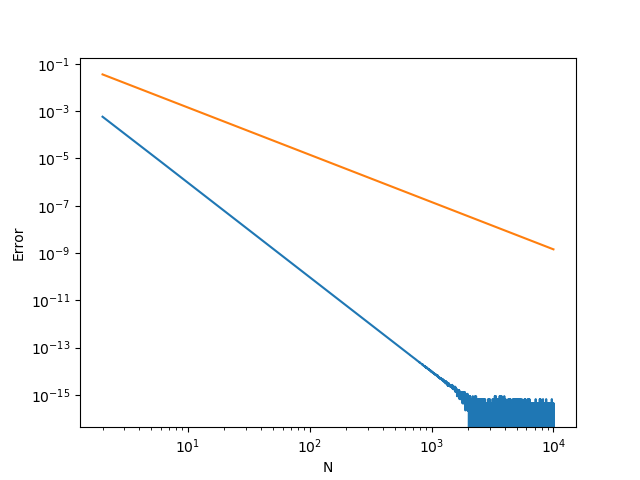
\includegraphics[width=\textwidth]{Ph20_Set2_Plot.png}

5.) The convergence plot does show the global error expected. This is because the global error of Simpson's Extended Formula is 4, while the global error of the Trapezoidal Rule is 2. These values are reflected in the slopes of the lines; the line corresponding to Simpson's Formula has slope -4 since the error decreases by $10^4$ as N decreases by 10, and the line corresponding to the Trapezoidal Rule has slope -2 since the error decreases by $10^2$ as N decreases by 10. \\
As one increases N to very large values, e.g., 5000, it becomes clear that the error stops decreasing. This is likely because there exists some limit on the accuracy with which the program knows the value of (e - 1). Therefore, the computer no longer knows whether or not the result is becoming closer to the true value, since it does not know the true value past a certain degree of precision. \\
\\
\\
7.) The Quad and Romberg methods are generally significantly more accurate than the Simpson's Rule and Trapezoidal Rule approximations for numerical integration. One manifestation of this is that the slope of their lines for the Error vs. N plot is steeper. 

\includegraphics[width=\textwidth]{Version Control Log.png}

\includegraphics[width=\textwidth]{MakefileSS.png}

\end{document}
